\section{Design of S-Aligner}
\label{Implementation}

This section describes the implementation of both the inter-CG and
intra-CG parallelism for the S-Aligner. Also discussed is our
bit-level encoding strategy and the exploitation of local device
memory.

\subsection{Large-Scale Inter-CG Parallelization}

\begin{figure}[!htb]
  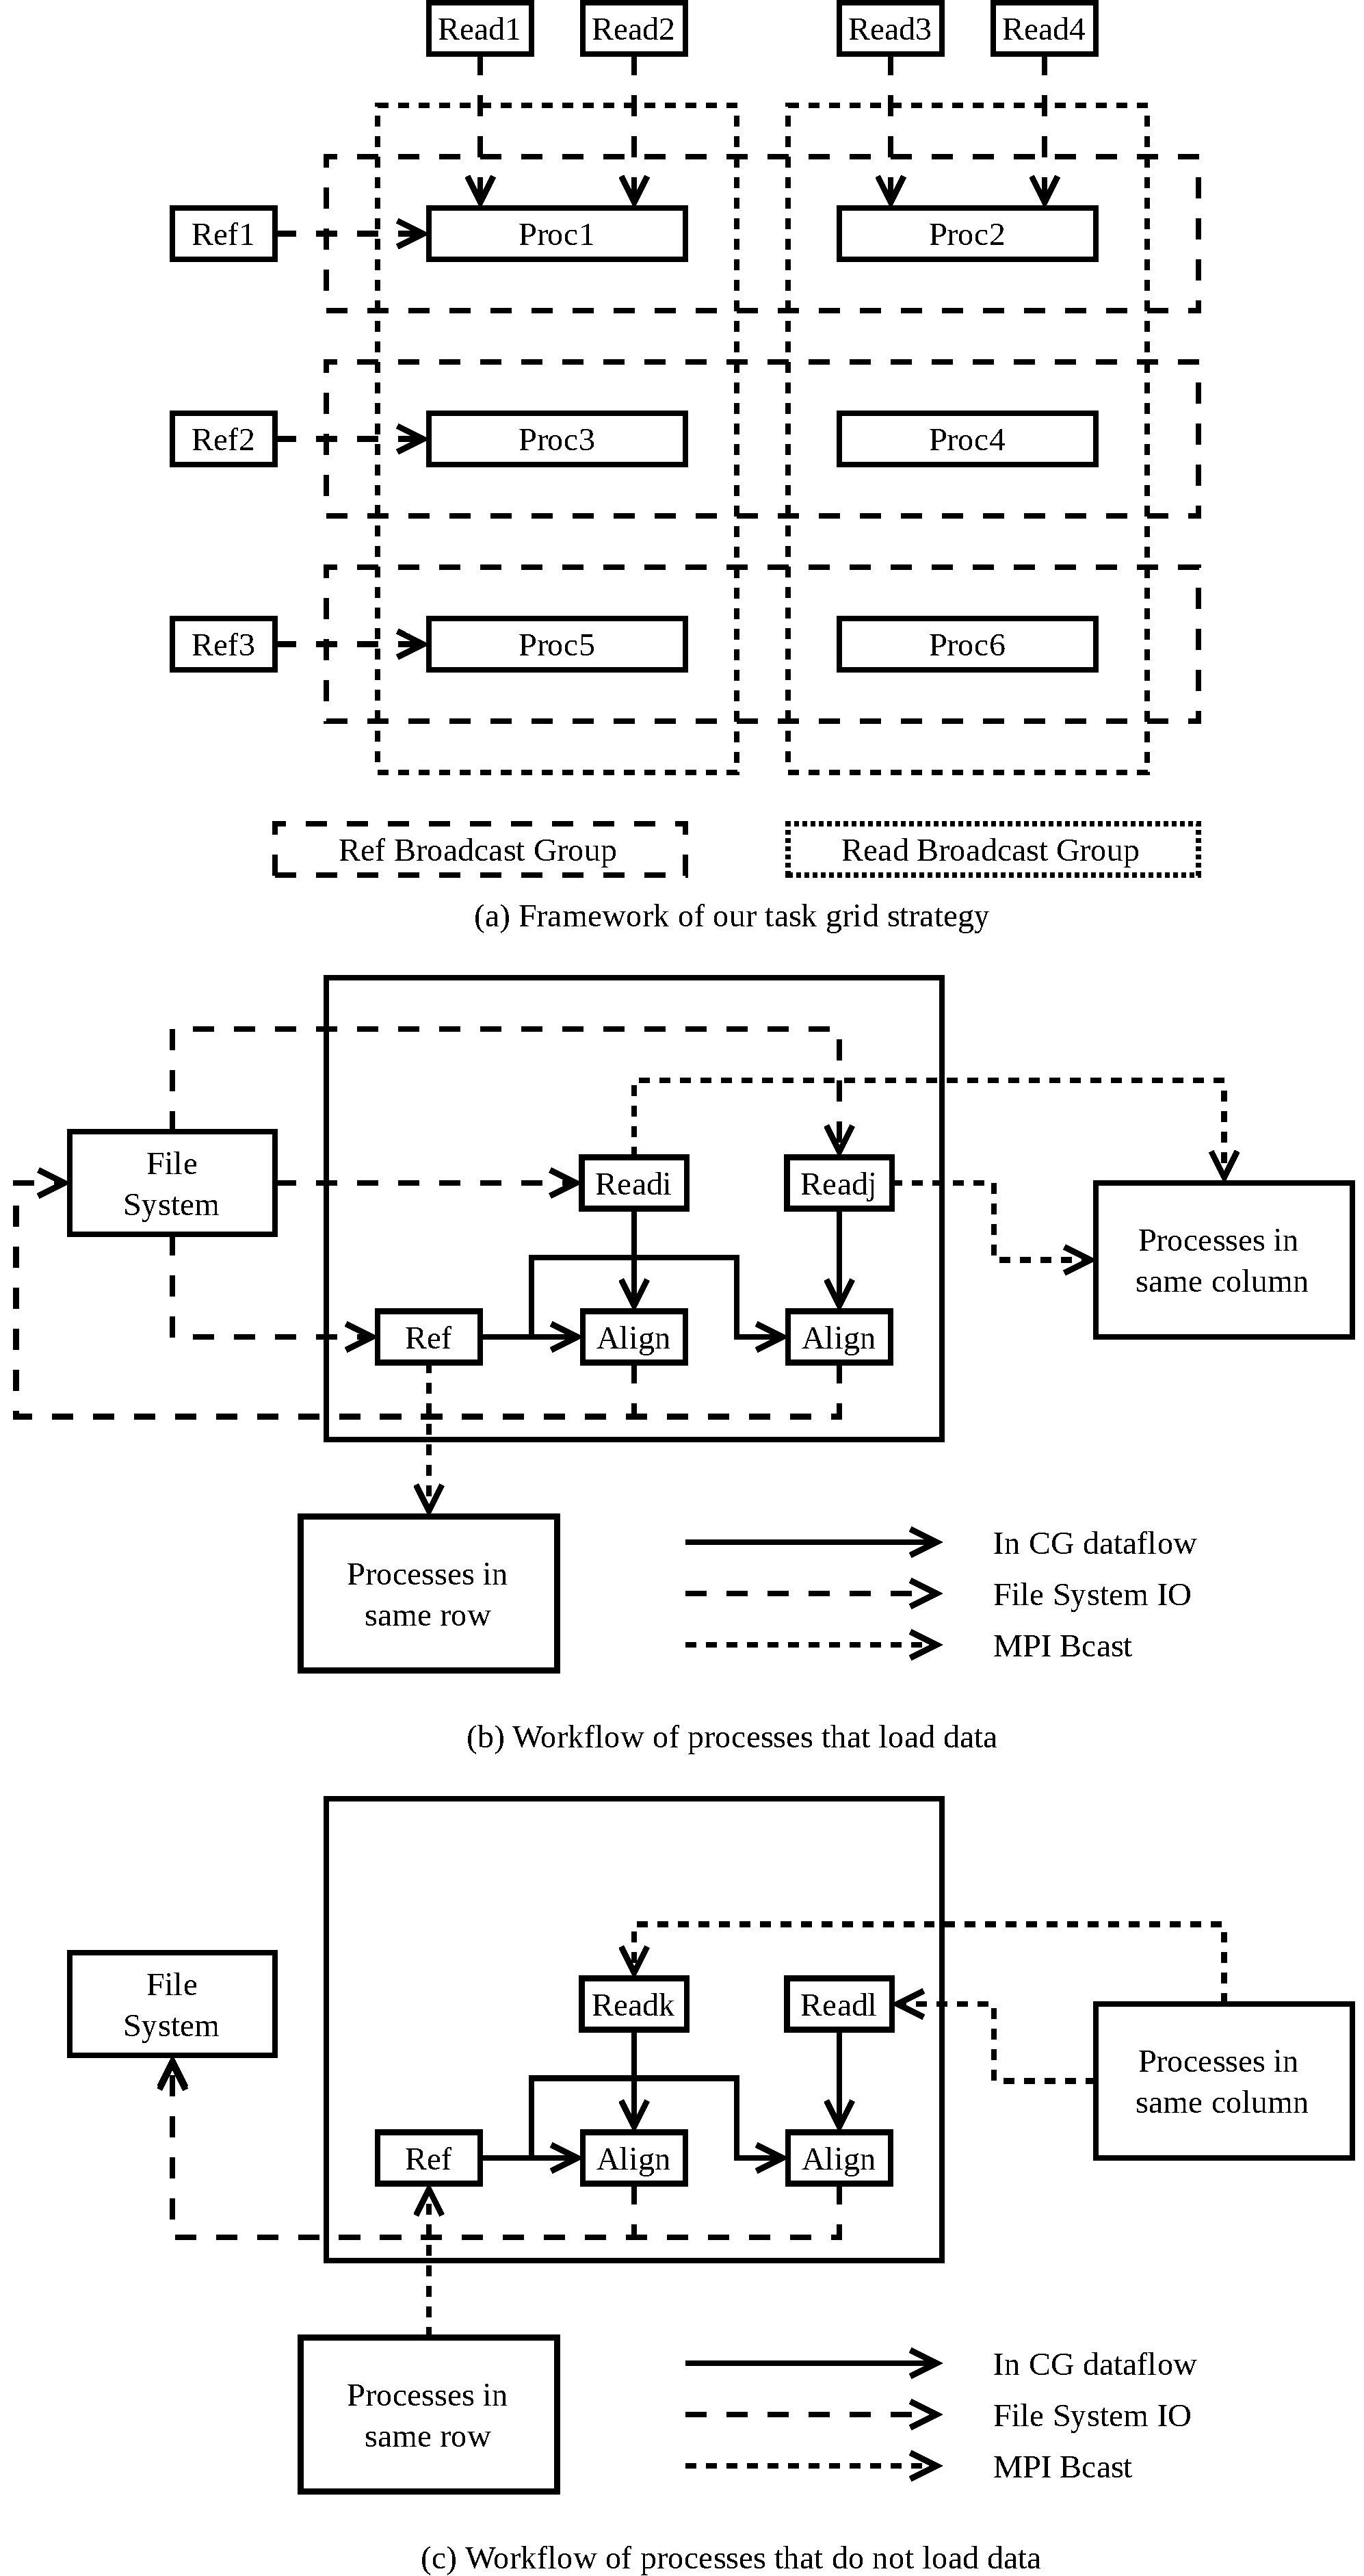
\includegraphics[width=\linewidth]{figures/GridNew}
  \caption{Our task-partitioning and file-loading strategy: (a)
    overall design; (b) and (c) detailed behavior of processes.}
  \label{TaskGrid}
\end{figure}

The highest level of parallelization employs a coarse-grained
partitioning scheme over a block distribution of reads and reference
genome using MPI. In our experiments we process up to 1.6 TB of read
data using up to 13,312 SW26010 nodes executing more than 50,000
dispatched processes. Thus, a na\"{\i}ve partitioning of the read file
into 50,000 pieces of approximately 32 MB size is not a suitable
solution because of the excessive data replication of the reference
genome index. Instead, we employ a partitioning strategy based on a
{\em task grid pattern} for the inter-CG parallelization by
concurrently assigning pairs of reference genome blocks and read
chunks to individual CGs. The two dimensions of the grid are spanned
by the reference block identifiers (rows) and read chunk identifiers
(columns) as shown in Figure \ref{TaskGrid}(a). Thus, processes in the
same row share a unique reference genome (index) block while processes
within a column use the same read chunk. Each process executes several
cells in one row in order to avoid replication of the relatively big
reference index.

\begin{figure}[!htb]
  \begin{center}
    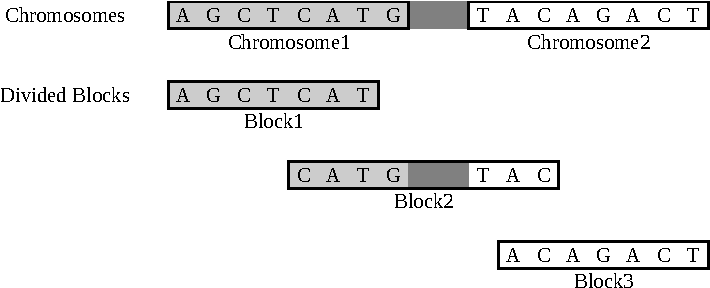
\includegraphics[width=0.9\linewidth]{figures/RefDiv}
    \caption{Exemplary partitioning of a reference genome based on
      concatenation and padded splits.}
    \label{RefDiv}
  \end{center}
\end{figure}

The read input file is partitioned into chunks of fixed size. This can
be easily achieved by splitting by lines. For the reference genome, we
first concatenate the individual chromosomes to form one long
string. We then divide it into blocks of suitable size according to
the memory capacity of a CG ($\approx$300 million bps per block). Note
that this partitioning scheme is disadvantageous when a chromosome is
scattered over two blocks or a read is mapped to the junction point of
two chromosomes. This issue can be resolved by padding `N's between
chromosomes. Moreover, when dividing a chromosome into two blocks, we
store several base pairs in a neighborhood around the break point in
both chunks. As a result, a read is always mapped correctly to a
contiguous region. Figure~\ref{RefDiv} depicts this approach.

The computing nodes of Sunway Taihu Light are connected to a network
file system via a 1 GBit/s interface, while the overall file system
bandwidth is $\sim290$ GB/s for the whole cluster. In practice,
efficient data distribution patterns have to be employed to reach
reasonable performance. The file system bandwidth is low compared with
the bisection bandwidth of $\sim70$ TB/s among compute nodes. To
address this issue, we employ a {\em group-and-broadcast} data reuse
strategy to avoid redundant file system accesses by sharing identical
data via Sunway's network among nodes. As tasks are assigned to grid
cells, we cluster processes working on the same reference genome block
to a row group ({\em ref broadcast group}), while processes working on
the same read chunk are clustered to a column group. If a process
calculates cells in the first row or first column ({\em read broadcast
  group}), it loads the corresponding reference block or read chunk
from the file system as shown in
Figure~\ref{TaskGrid}(b). Subsequently, it broadcasts the loaded data
to processes calculating the same row or column, while the other
processes wait for the broadcast data as shown in
Figure~\ref{TaskGrid}(c). After the data-loading stage, processes can
perform their computation concurrently.

\begin{figure}[!htb]
  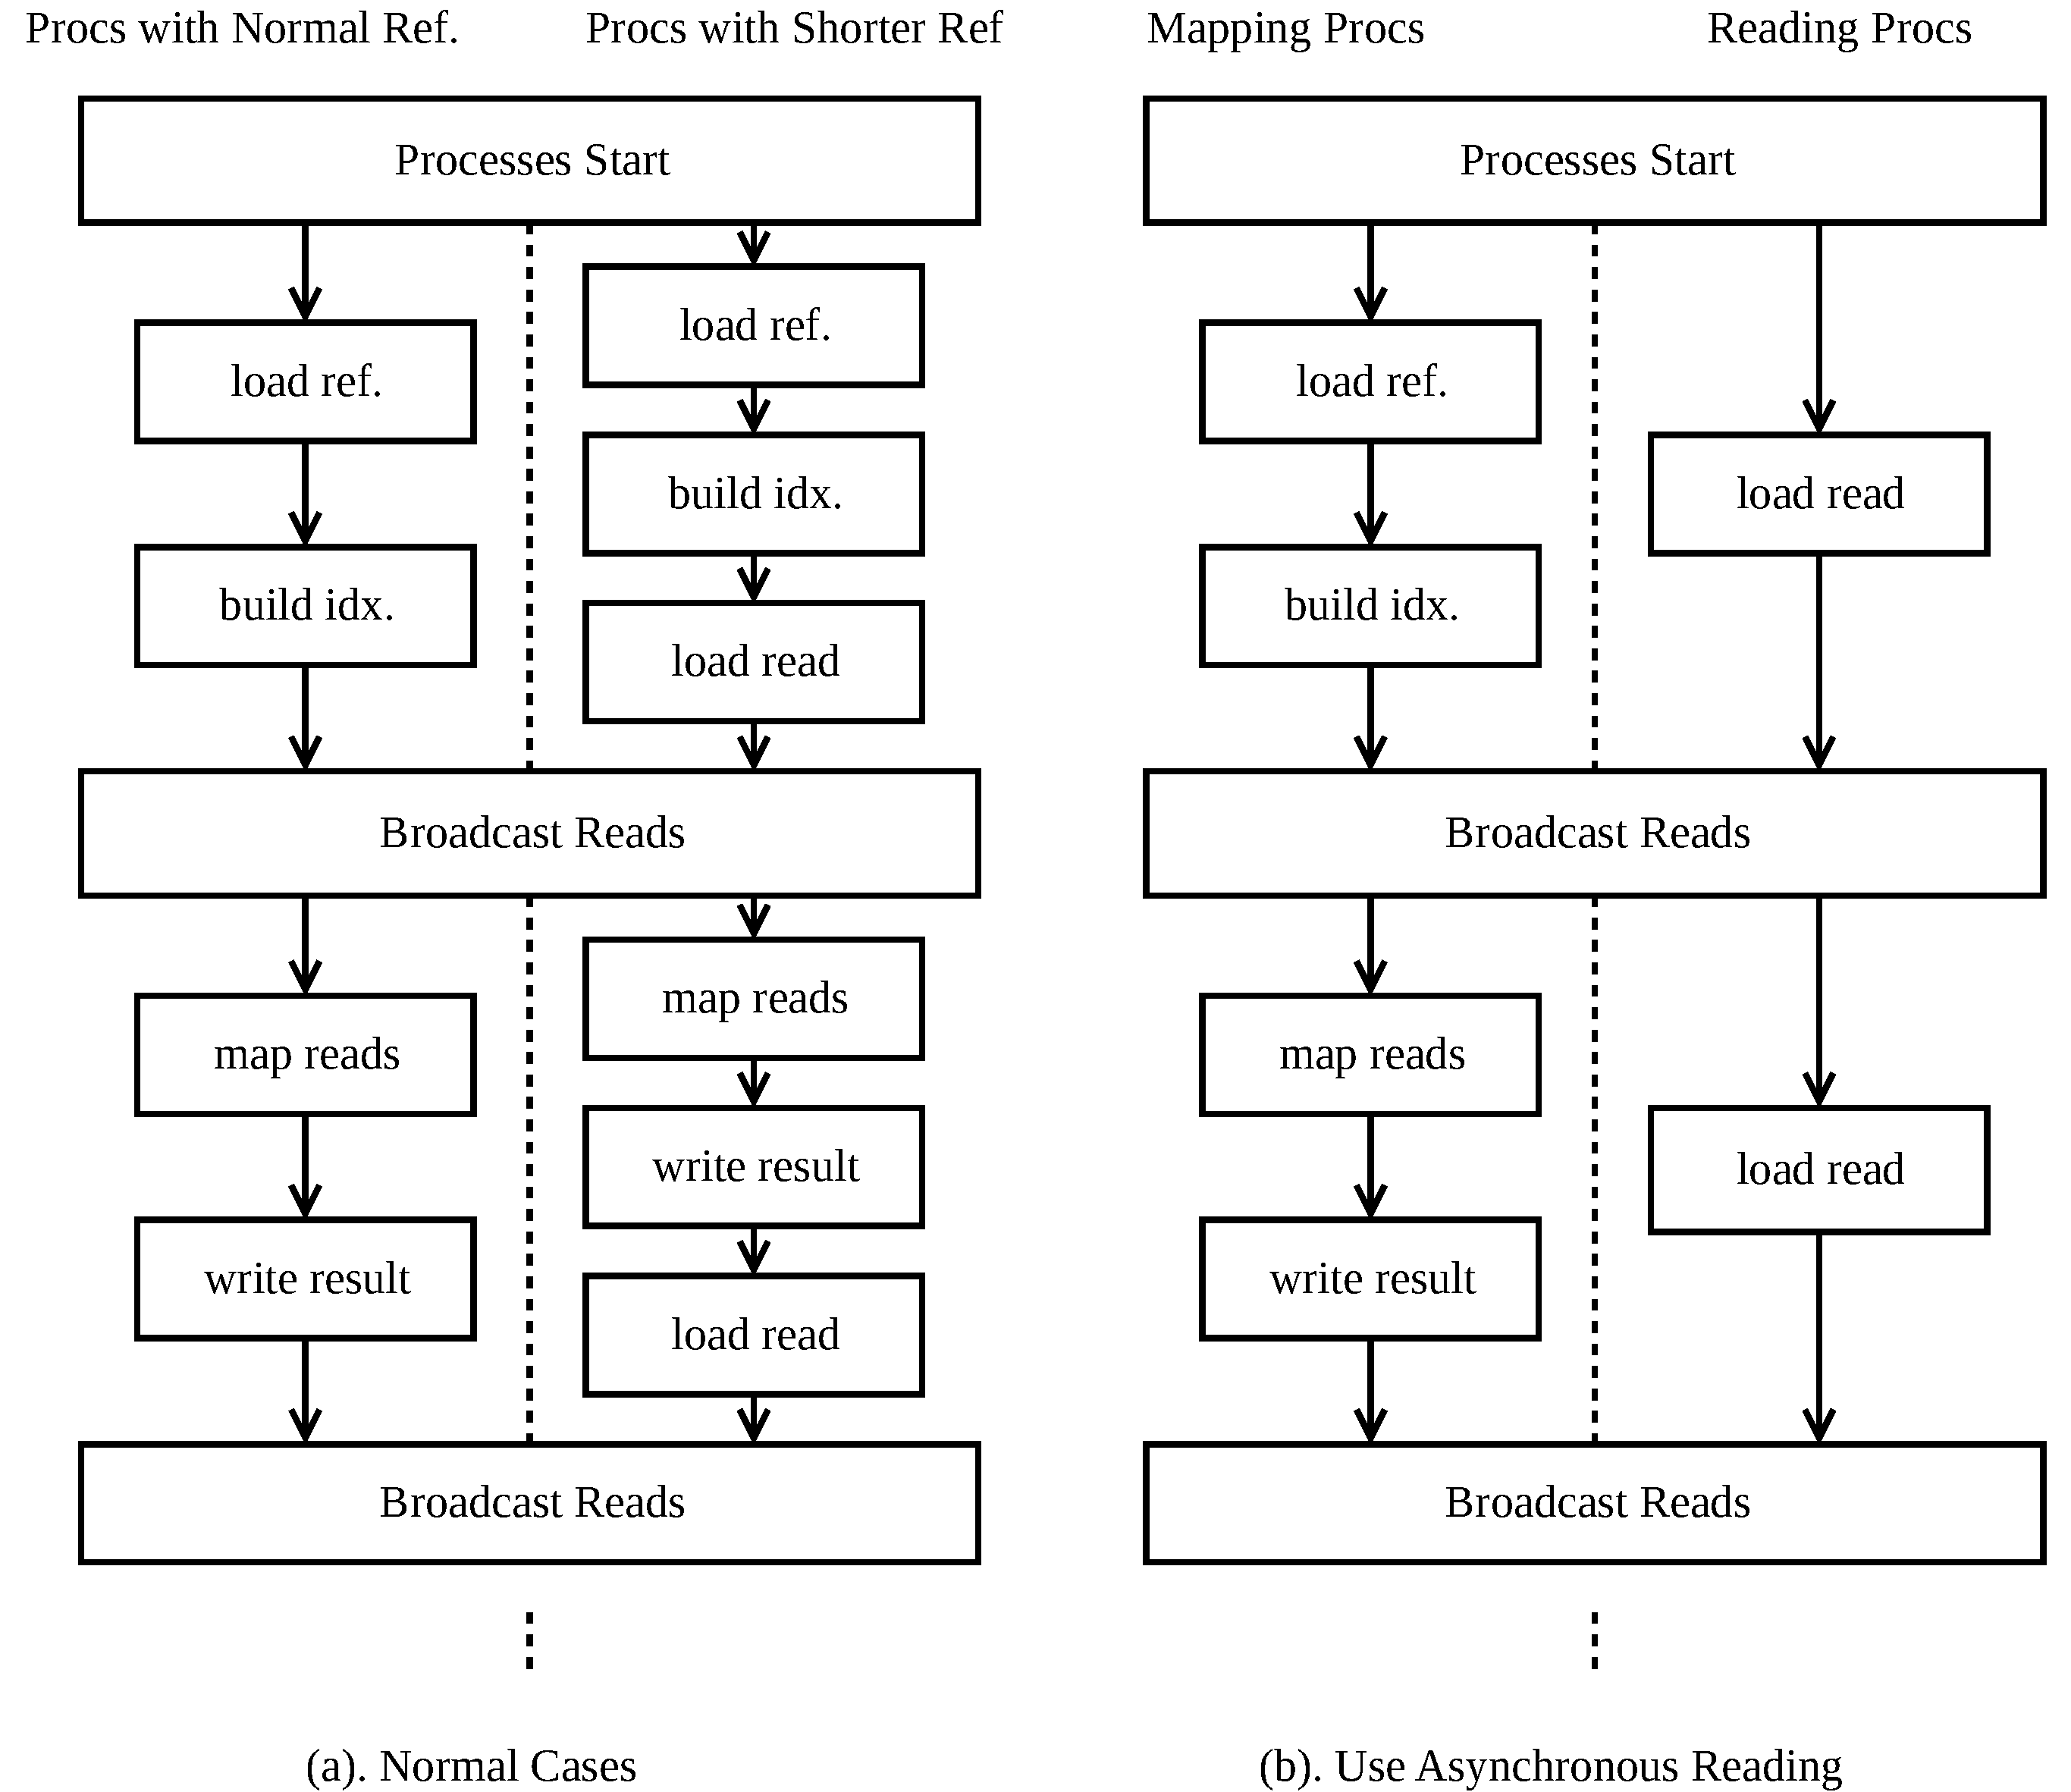
\includegraphics[width=\linewidth]{figures/AsyncRead}
  \caption{Asynchronous data loading strategy: (a) default case, and
    (b) case when there is no significantly shorter reference block.}
  \label{AsyncRead}
\end{figure}

Our reference genome partitioning strategy illustrated in
Figure~\ref{RefDiv} often generates one reference genome block that is
significantly shorter than the others. This block is assigned to the
first row of our task grid. Thus, processes in the first row take less
time during computation and will have sufficient time to load reads
for the subsequent round of computation. This approach therefore
reduces the idle time of other processes waiting for read data.
Figure \ref{AsyncRead}(a) illustrates this strategy.

We further provide an optional asynchronous data-loading strategy in
case that there is no significantly shorter reference block. In this
case we add a row of processes that loads only reads. When other
processes in the column are computing alignments, these processes
exclusively load new read chunks. After loading and computation have
been completed, all processes within a column receive the loaded data
by means of an \texttt{MPI\textunderscore Bcast}. In our experiments,
this approach reduces the idle time between computing two read chunks
by over 90\% when using 8 processes. Figure \ref{AsyncRead}(b)
illustrates this strategy.

\subsection{Multithreaded Intra-CG Parallelization}

\begin{figure}[!htb]
  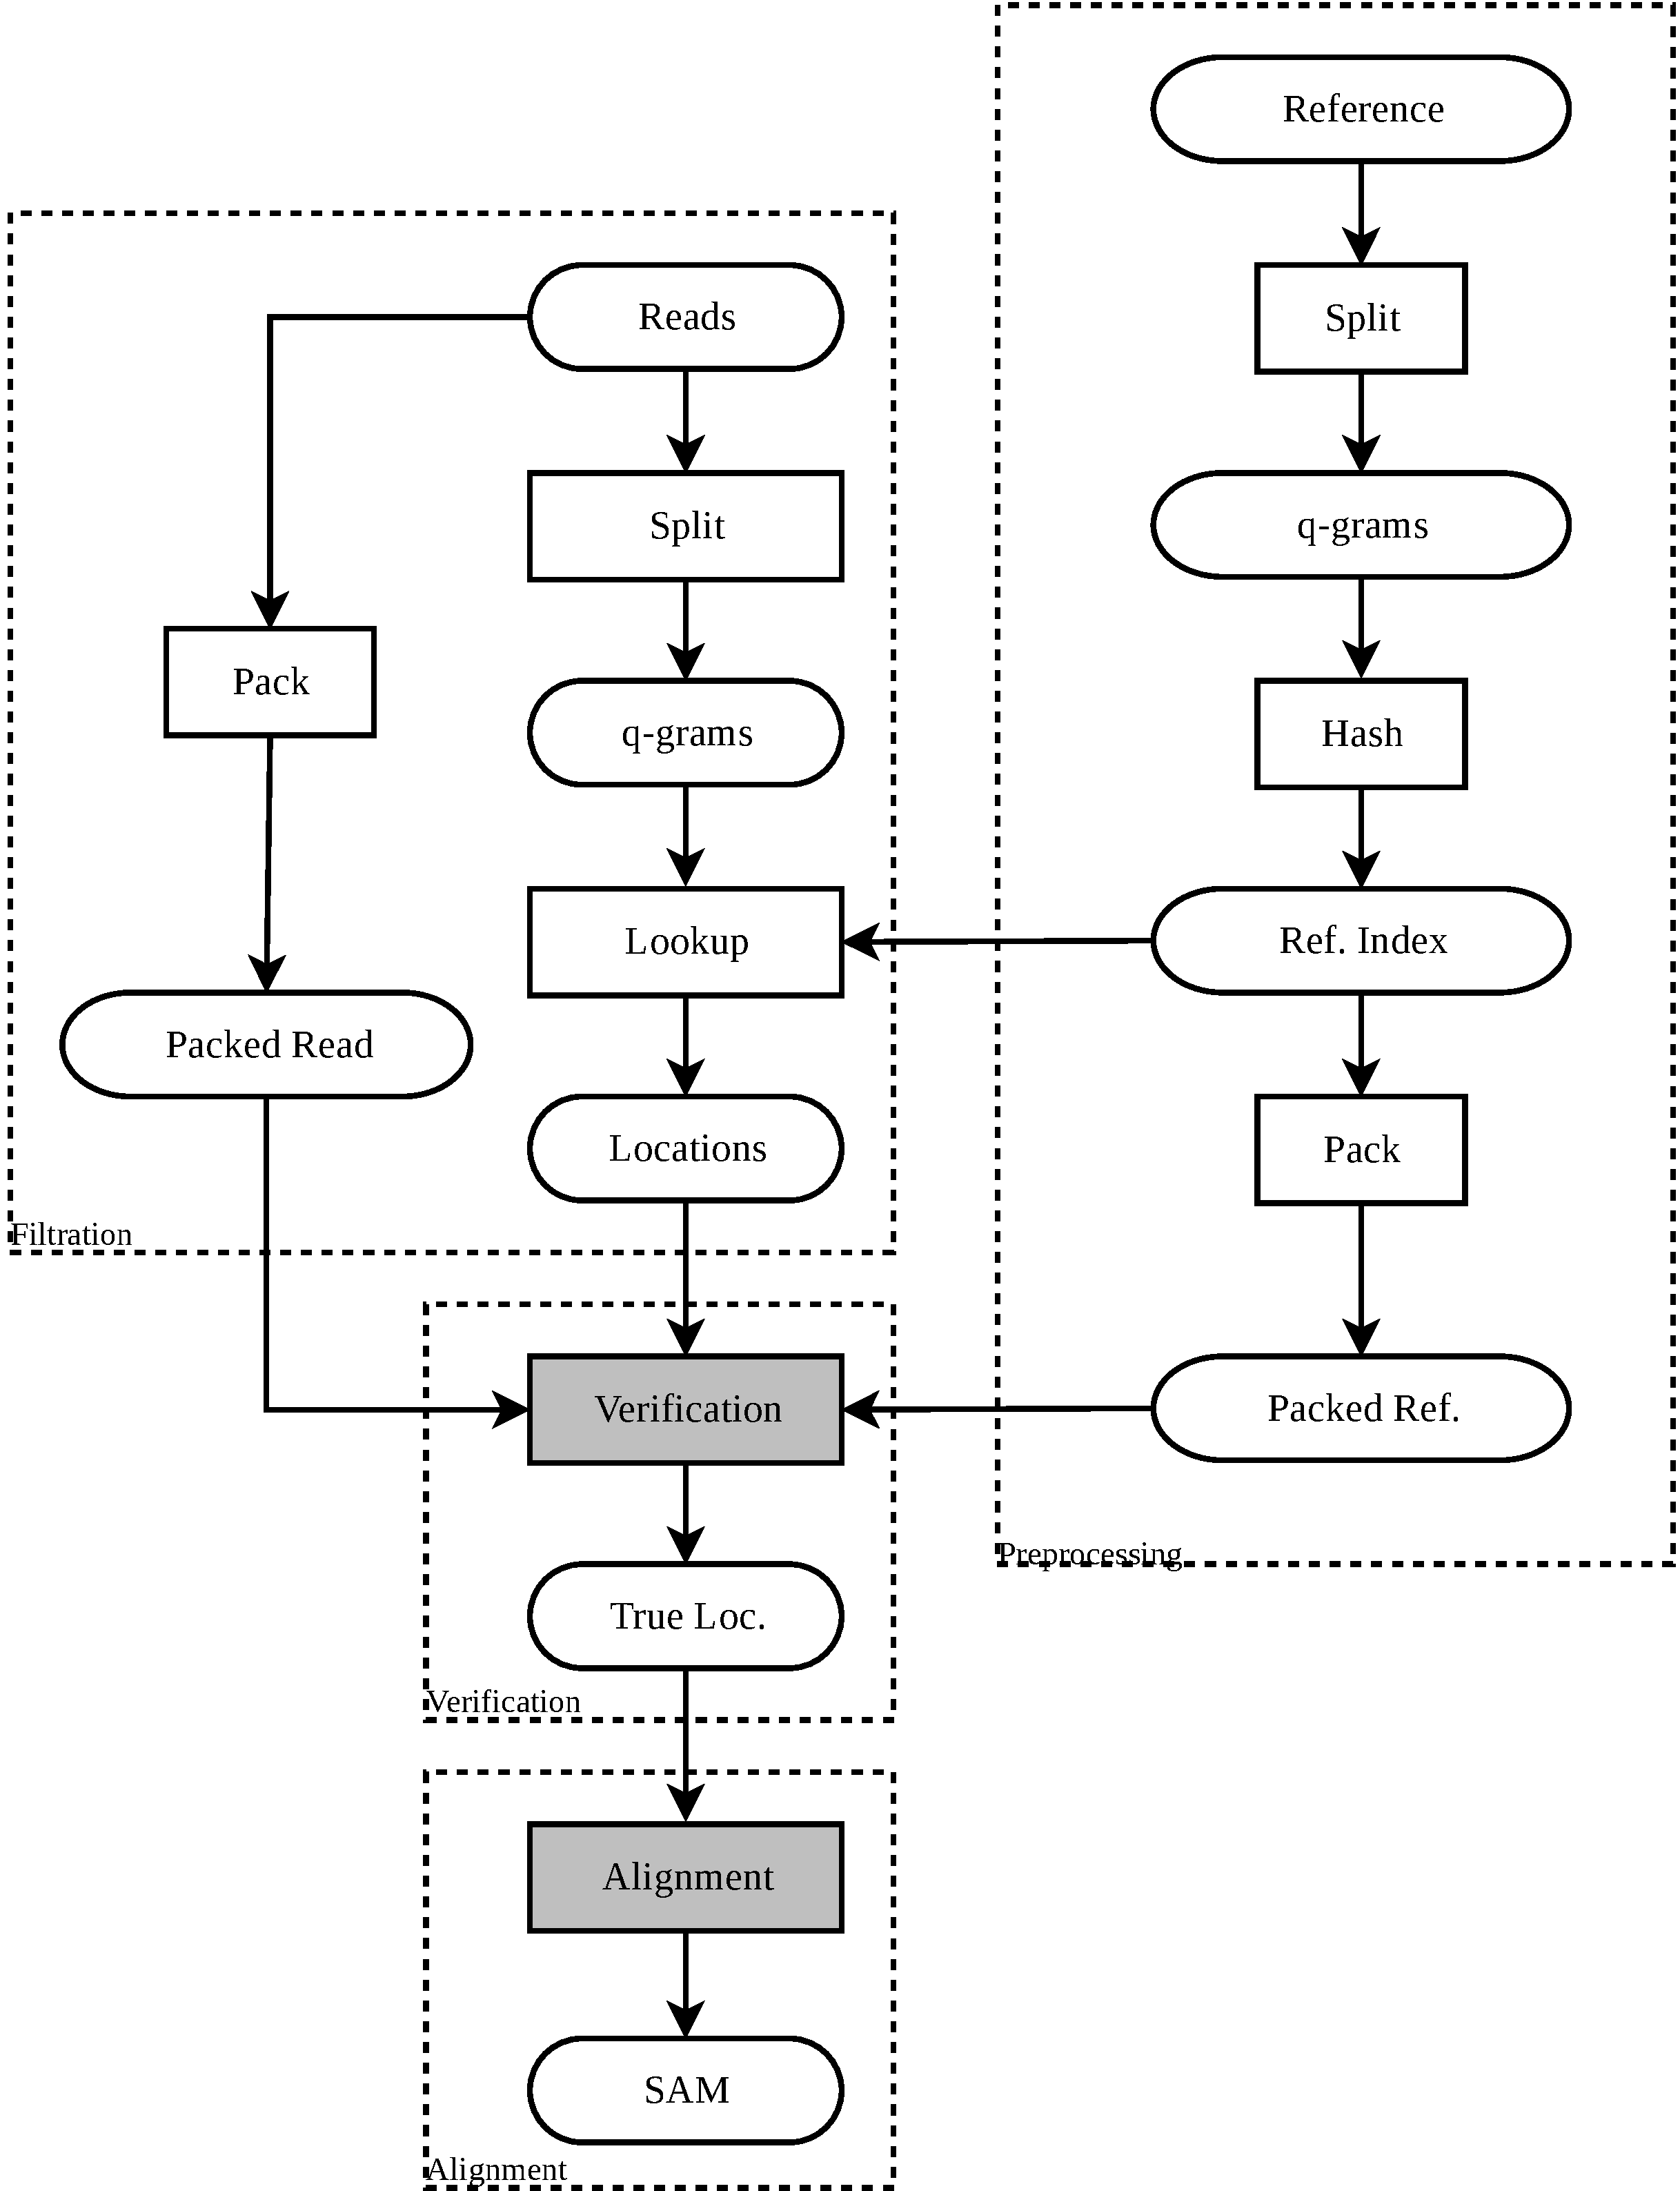
\includegraphics[width=1\linewidth]{figures/FrmWk}
  \caption{Workflow of S-Aligner on a single CG: gray boxes correspond
    to tasks assigned to SPs while tasks in white boxes are executed
    on the MP.}
  \label{FrmWk}
\end{figure}

The second level of parallelism exploits the threading capabilities of
a CG. Our design within a single node is a comprehensive read mapper
based on the described seed-and-extend approach using the three-stage
pipeline: filtration, verification, and alignment. The filtration step
uses a look-up table of $q$-grams of the assigned reference genome
block that can be loaded from a preprocessed index file or
alternatively calculated on-the-fly by a radix sort-based hash table
construction method. After the MP performs the lookup of each
non-overlapping $q$-gram of a read, it stores the retrieved intervals
in a SIMD-friendly manner allowing for efficient vectorization during
the subsequent verification step on the SPs. Verification selects all
intervals that comply with the restricted edit distance using Myers'
bit-parallel algorithm. Afterwards, we employ a banded version of the
Smith-Waterman algorithm on the SPs to align the remaining intervals
that have passed verification. Figure~\ref{FrmWk} shows the workflow
of our intra-CG implementation.

\begin{figure}[!htb]
  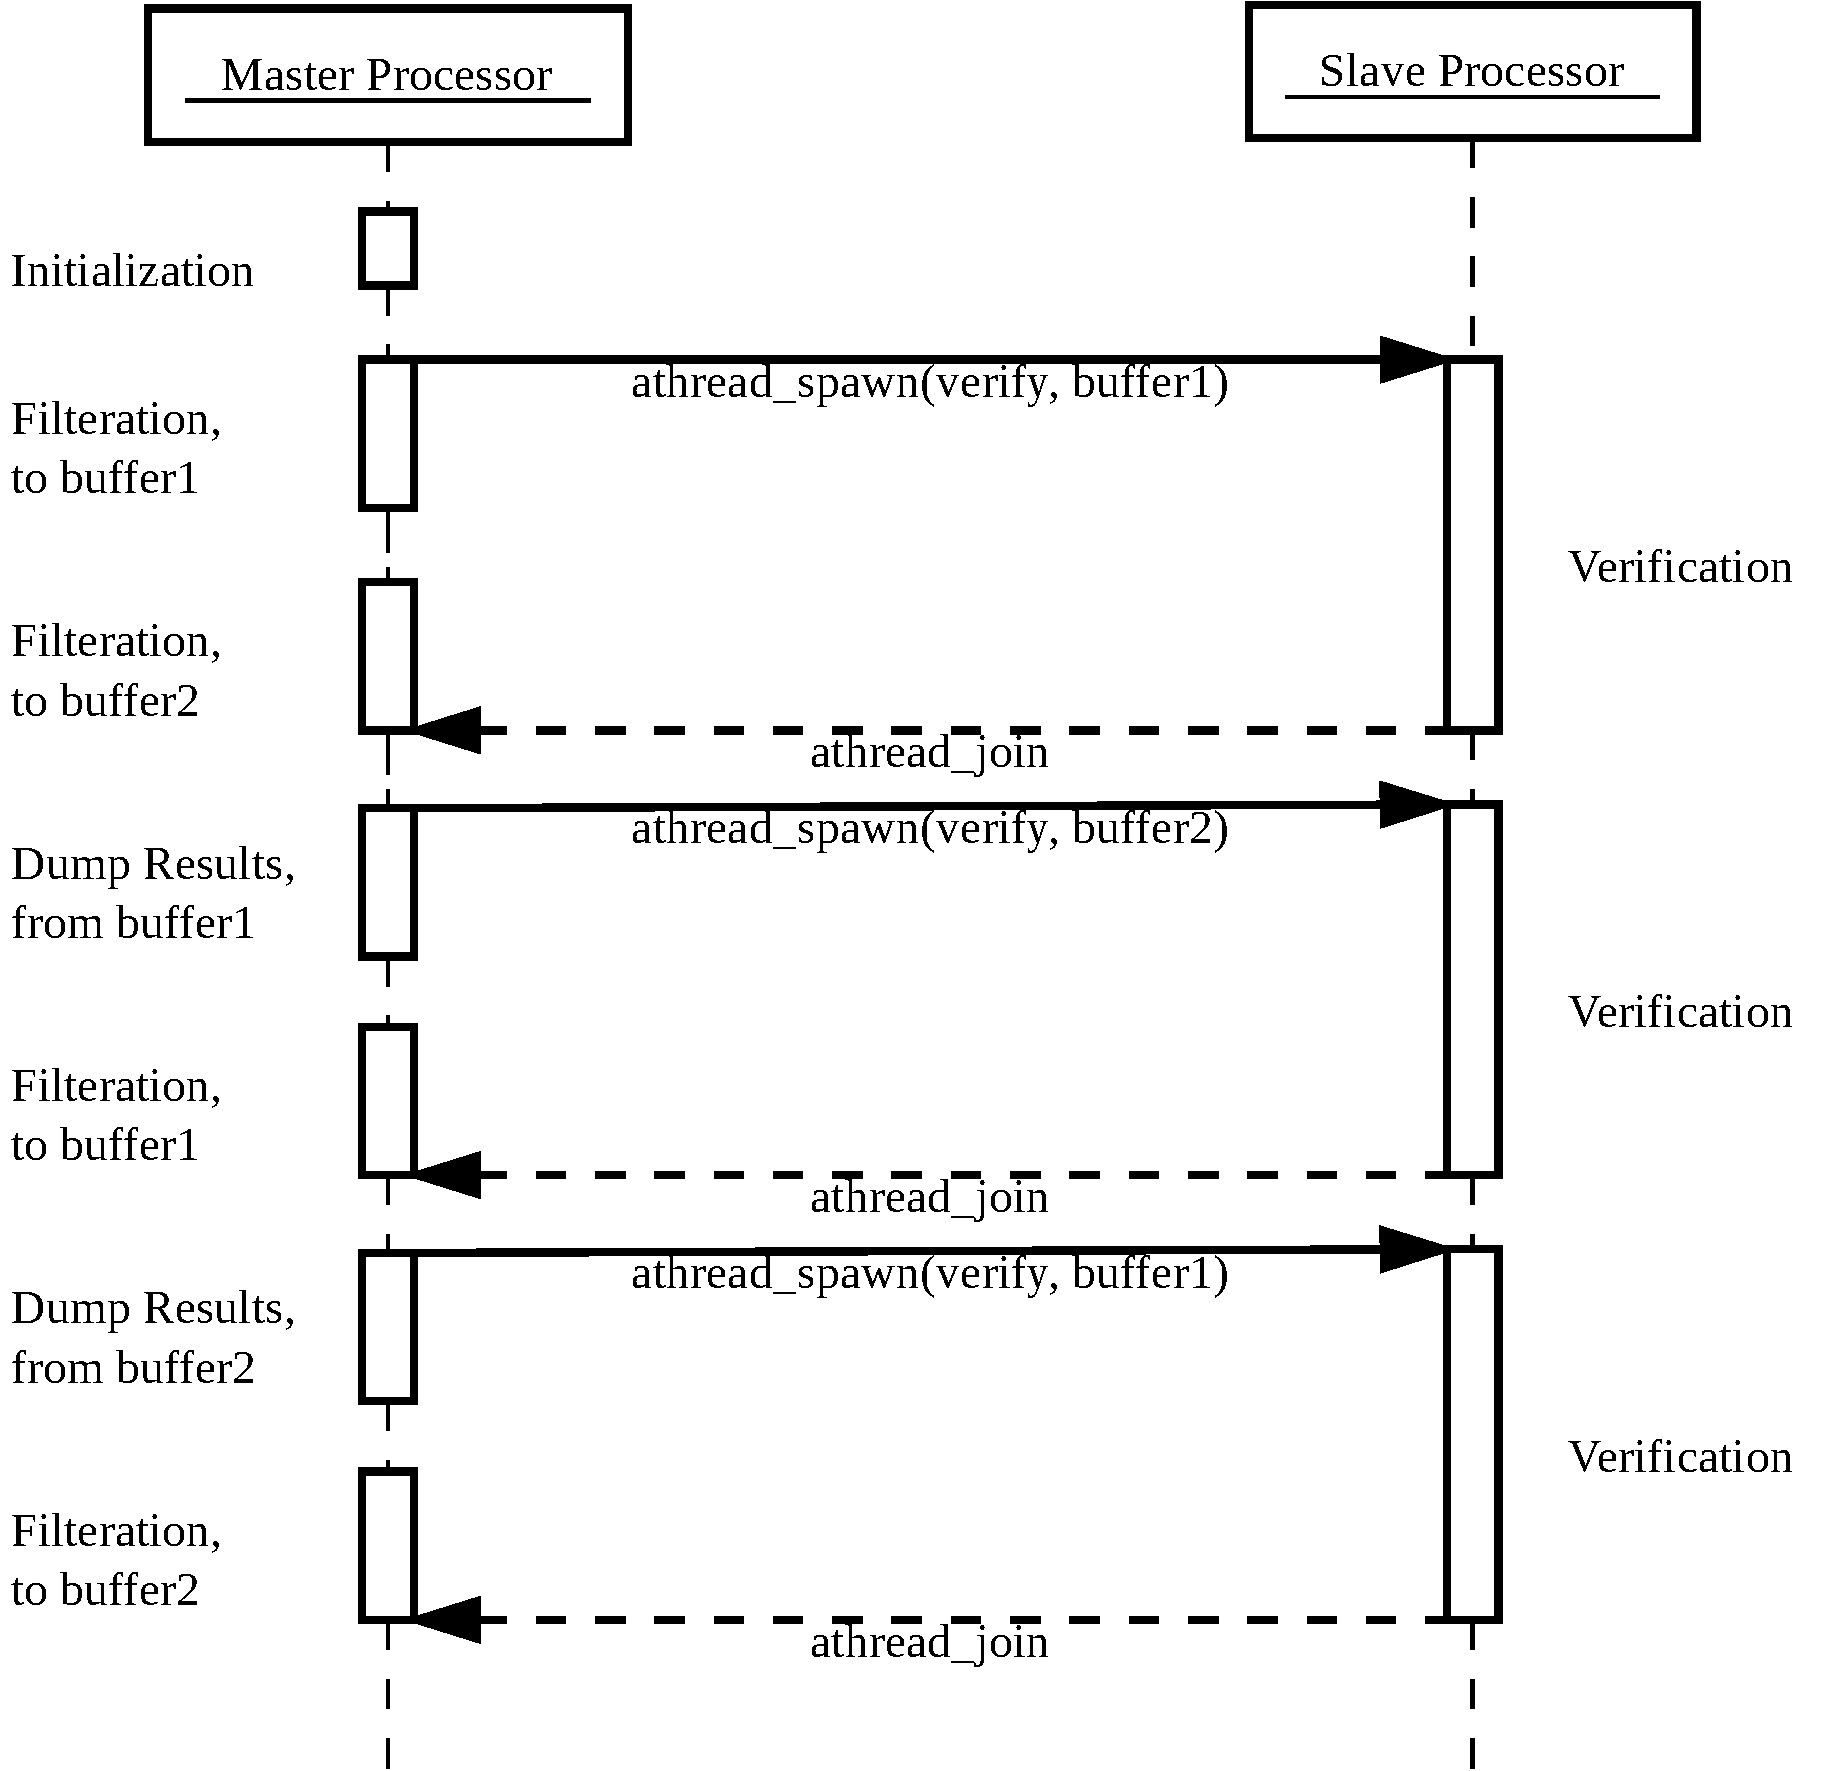
\includegraphics[width=1\linewidth]{figures/AsyncPara}
  \caption{Asynchronous filtration.}
  \label{AsyncPara}
\end{figure}

The intra-CG parallelization is realized by a task parallelization
scheme implemented using spawn and join calls of the {\em athread}
library. The MP executes the filtration stage while the SPs process
the verification step. Each read is divided into non-overlapping
$q$-grams. The MP looks up those $q$-grams in the reference genome
index and returns a number of intervals. The MP copies them to a
buffer that is transferred to the LDM of SPs for verification. We
employ a dual buffer strategy by allocating two buffers for storing
the intervals identified by the MP. When the MP has finished filling
one buffer, it waits for the SP thread group to join, and then
dispatches an SP thread group to verify these intervals. Subsequently,
the MP fills another buffer, while the SP thread group performs
verification. These steps are repeated until all reads are processed
(see Figure \ref{AsyncPara}). The dual buffer strategy reduces the
idle times of SPs and is also used for implementing the subsequent
alignment stage.

\begin{figure}[!htb]
  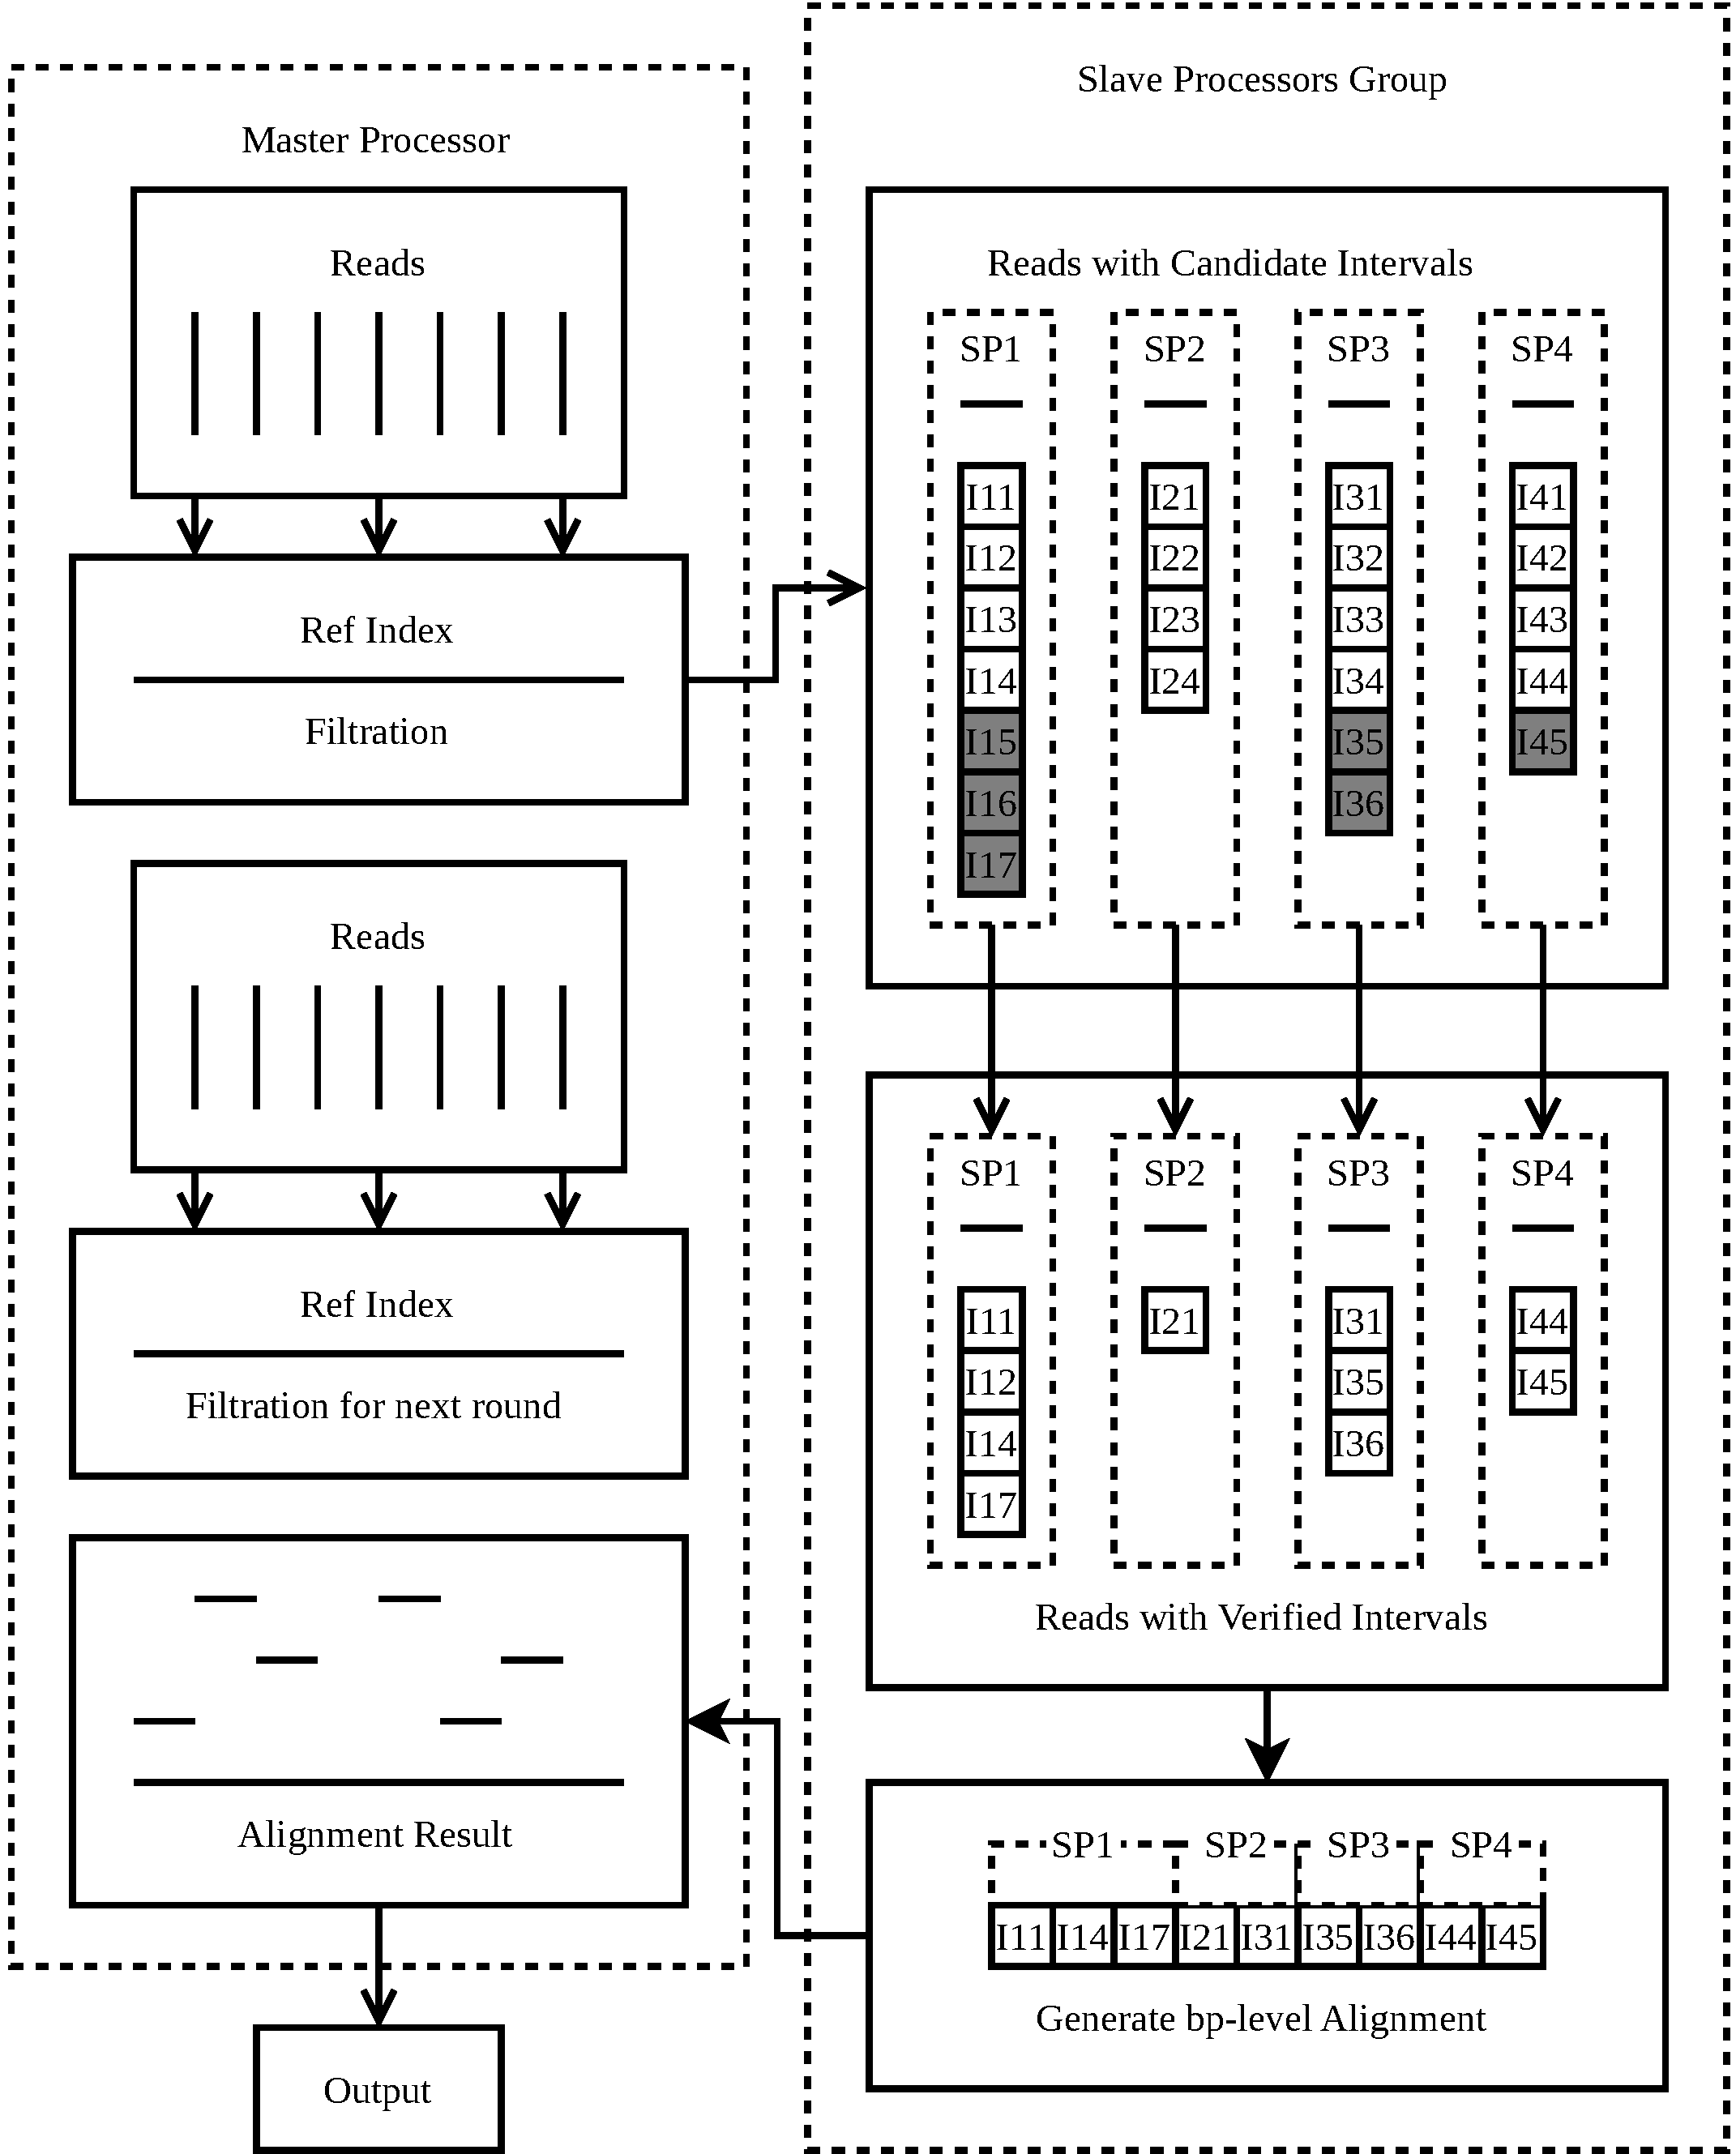
\includegraphics[width=\linewidth]{figures/SPParallel}
  \caption{Framework of our parallelization scheme within one CG: the
    MP performs filtration and output of alignment results while SPs
    verify identified candidate locations and generate base-pair level
    alignments. Gray boxes indicate the intervals verified in the
    second round of verification (assuming $slice\_num = 4$).}
  \label{SPParallel}
\end{figure}

Figure~\ref{SPParallel} illustrates our framework for dividing the
computation between the MP and SPs within a single CG. The number of
seeds identified for a given read can vary while the verification time
of a single seed is constant. Thus, a simple static assignment of seed
intervals per read to SPs can cause workload imbalance.  To balance
the workload, we introduce the parameter $slice\_num$, which restricts
the maximum number of seed intervals to be verified for one read. If
there are more than $slice\_num$ seed intervals to be verified for a
read, we spawn verification threads with the first $slice\_num$
intervals. The remaining intervals will be verified in a subsequent
round of spawns. A value of $slice\_num$ that is too large can reduce
the overhead of spawning SP thread groups, but it worsens workload
balance, and vice versa. Our default value of $slice\_num = 100$
provides a good trade-off in practice.


\subsection{SIMD Vectorization}

Implementing Myers' bit-parallel algorithm using ShenWei's SIMD
intrinsics requires a bit-level encoding of DNA sequences to
efficiently evaluate the characteristic function $\chi(s_{i-1} =
s'_{j-1})$ for all $i, j$.

Different approaches have been used in existing aligners: BWA
\cite{bwa} employs an {\em array of structures} (AoS) while RazerS3
\cite{razers3} stores a DNA sequence in a profile using one-hot
encoding. While the AoS approach is more space-efficient and
cache-friendly, the usage of a profile with one-hot encoding supports
bit-parallel computation in a more efficient way.  Because of the
small size of the LDM and the requirement of bit parallelism, we
employ an encoding strategy that combines an AoS with an SoA ({\em
  structure of arrays}) approach, which we call an AoSoA ({\em array
  of structures of arrays}). This mixed strategy builds two
bit-vectors in an interleaved fashion. Thus, we can fetch the encoded
sequence by one DMA-intrinsic and calculate $\chi(s_{i-1} = s'_{j-1})$
in terms of two logical equality operations. Figure~\ref{MixPack}
illustrates the encoding strategy.

\begin{figure}[!htb]
  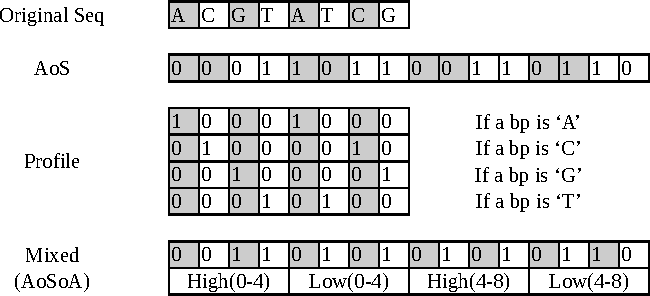
\includegraphics[width=0.9\linewidth]{figures/MixPack}
  \caption{Bit-level encoding strategies for DNA sequences. For
    simplicity, we use a 4-bit word instead of 64-bit word for
    illustrating our combined AoSoA strategy (bottom).}
  \label{MixPack}
\end{figure}

When updating the five bit-vectors according to
Equation~\ref{one-hot-myers} along the columns in a bit-parallel
fashion, a circular dependency needs to be resolved: $D^0_{i,j}$
depends on $H^-_{i-1, j}$, which in turn depends on $D^0_{i-1,j}$ (a
value we have not computed yet). Myers \cite{myers} has shown that
this can be solved by using logical operations and an
addition. ShenWei's SIMD instructions support 256-bit integer
arithmetic, such as \texttt{simd\_uaddo\_take\_carry} (short for SIMD
unsigned octa-word add, taking carry) which adds two 256-bit operands
and returns a 256-bit unsigned integer. Thus, different from
implementations of Myers' algorithm on other architectures (e.g.,
\cite{chacon}), our implementation does not require additional
instructions to process carries generated within a SIMD
lane. Unfortunately, there is no 256-bit compare instruction. Thus, we
have implemented comparisons in terms of shifting operations.

Furthermore, we have simplified the core loop as much as possible in
order to avoid branching statements. This action results in an
implementation consisting of 23 intrinsics as shown in Figure
\ref{cores}, where \texttt{resi32} is set to $|read|\mod 32 - 1$.

\begin{figure}[!htb]
    \begin{lstlisting}[frame=single, xleftmargin=3.5ex]
t1    = simd_vxorw(ref_hi,read_hi[k]);
t2    = simd_vxorw(ref_lo,read_lo[k]);
X     = simd_vbisw(t1,t2); 
X     = simd_vxorw(X,one); 
X     = simd_vbisw(X,VP[k]);
D0    = simd_vandw(X,VP[k]);
D0    = simd_uaddo_take_carry(D0,VP[k]);
D0    = simd_vandw(D0,VP[k]);
D0    = simd_vandw(D0,X);
HN    = simd_vandw(VP[k],D0);
HP    = simd_vbisw(VP[k],D0);
HP    = simd_vxorw(HP,one);
HP    = simd_vbisw(HP,VN[k]);	
X     = simd_sllow(HP,resi32);
X     = simd_vbisw(X,pr_HP);
pr_HP = simd_srlow(HP,255);
VN[k] = simd_vandw(X,D0);
VP[k] = simd_vbisw(X,D0);
VP[k] = simd_vxorw(VP[k],one);
t2    = simd_sllow(HN,resi32);
t2    = simd_vbisw(t2,pr_HN);
pr_HN = simd_srlow(HN,255);
VP[k] = simd_vbisw(t2,VP[k]);	
    \end{lstlisting}
    \caption{SIMD core instructions used to implement Myers' algorithm
      on ShenWei. The reference sequence is presented as
      \texttt{ref\_hi}, the high-bit of the pattern, and
      \texttt{ref\_lo}, the low-bit of the pattern. The read sequence
      is stored in the vectors \texttt{read\_hi[k]} and
      \texttt{read\_lo[k]}. The variables \texttt{D0}, \texttt{HN},
      \texttt{HP}, \texttt{VN}, \texttt{VP} refer to the corresponding
      variables in Equation~\ref{one-hot-myers}.}
    \label{cores}
\end{figure}

\subsection{Exploiting Local Device Memory}

\begin{figure}[!htb]
  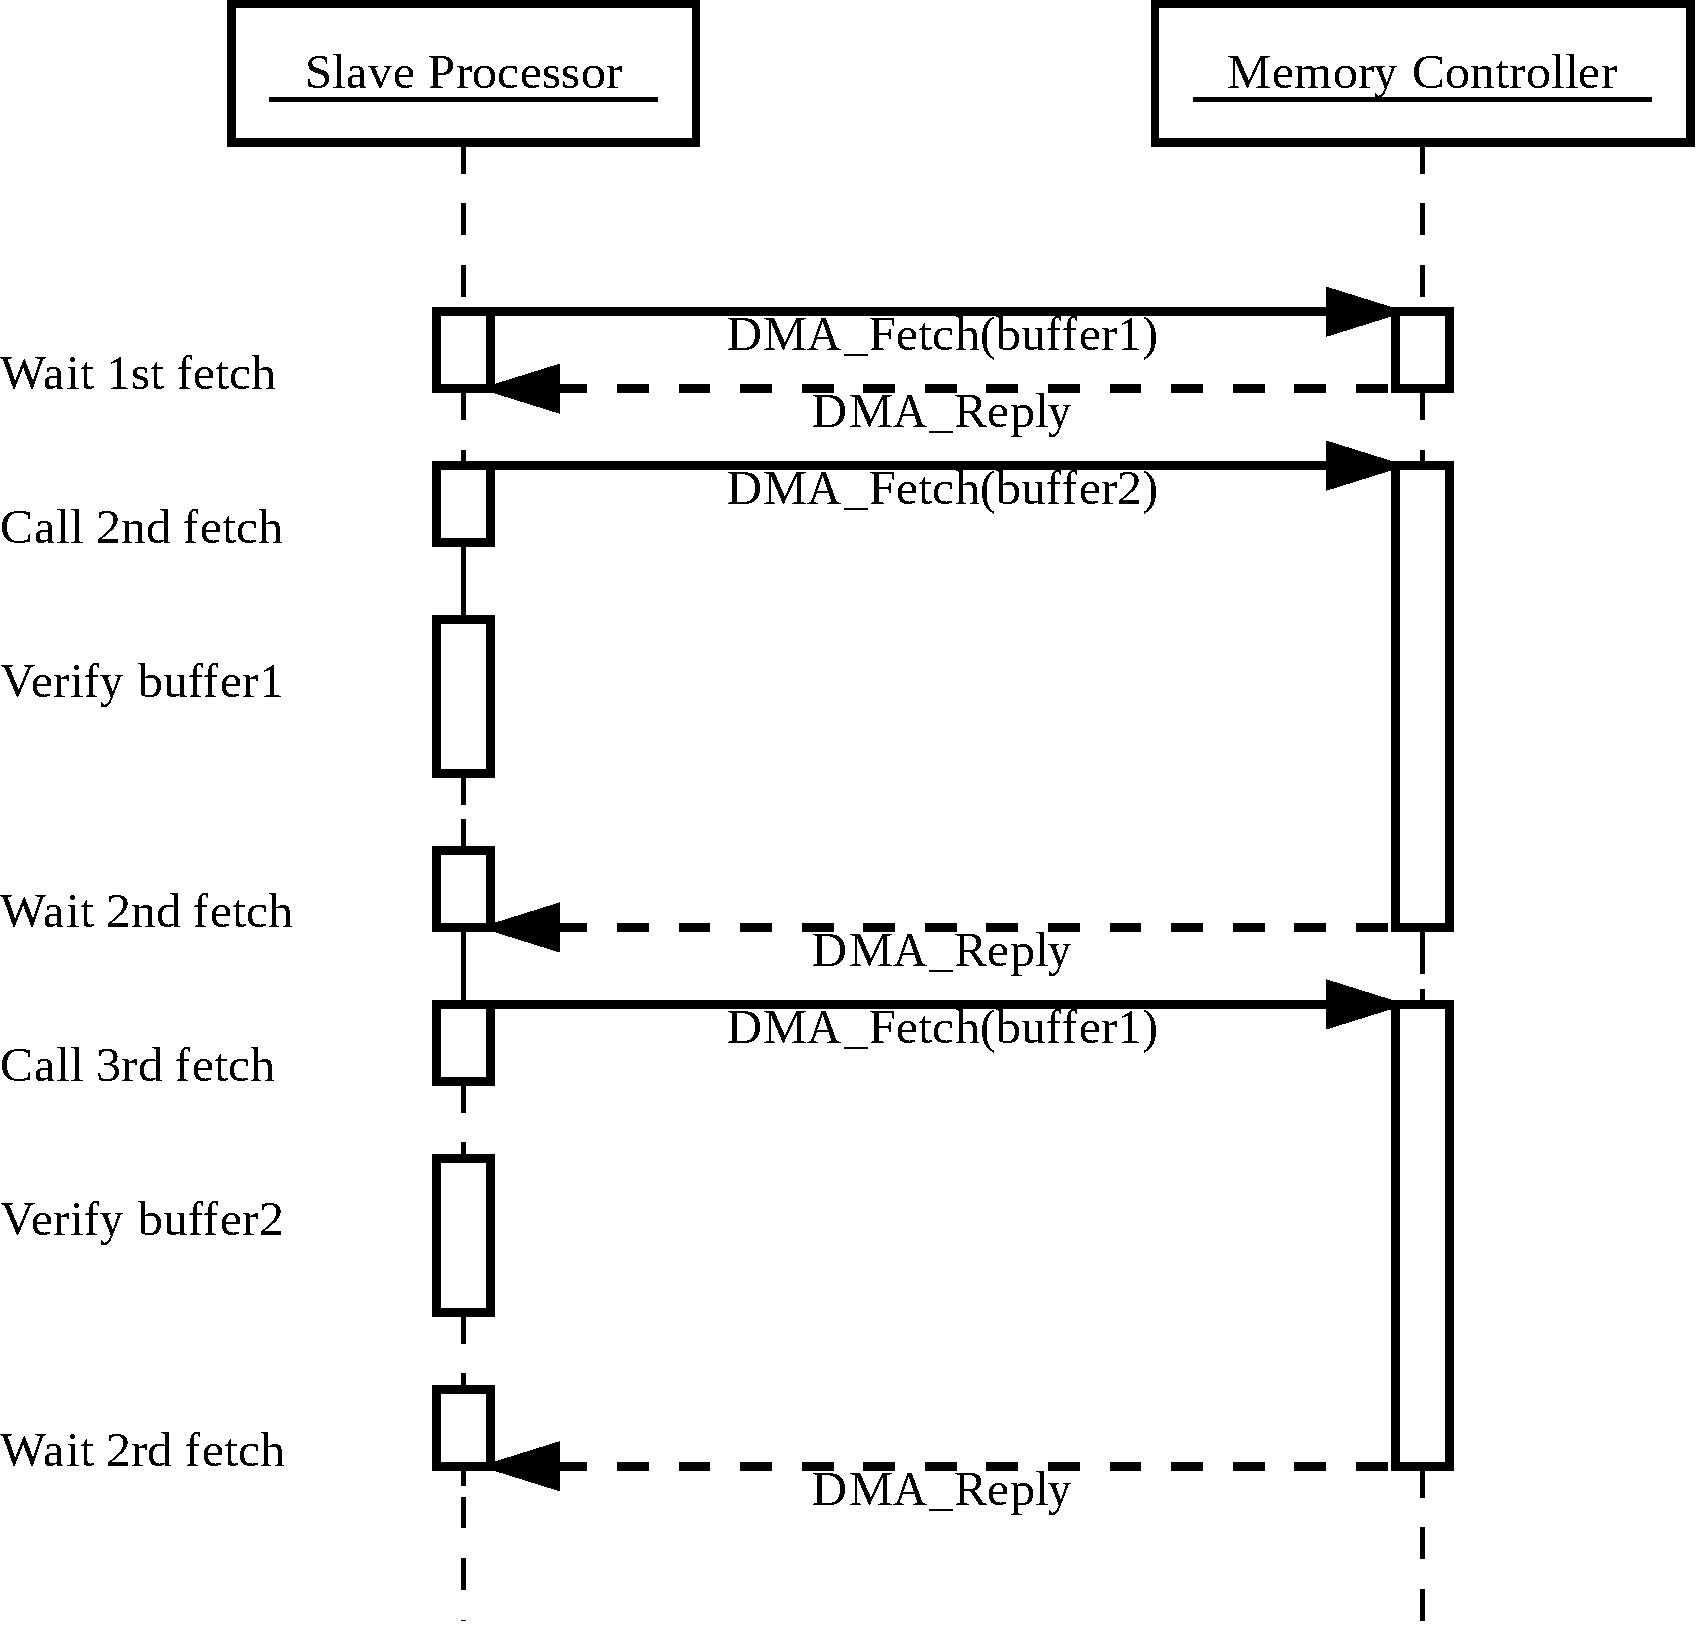
\includegraphics[width=1\linewidth]{figures/AsyncTrans}
  \caption{Asynchronous data transfer to LDM.}
  \label{AsyncTrans}
\end{figure}

Since SPs do not have any cache and the latency to access the DDR3
shared memory is high, the usage of the explicitly managed LDM is
crucial.  DMA fetching is the most efficient way to transfer data
between main memory and LDM (i.e., significantly faster than using
functions such as \texttt{memcpy}). DMA calls are handled by the
memory controller, and SPs can continue to perform computation. Thus,
we can overlap data transfers from shared memory to LDM and the
verification of intervals using Myers' algorithm by using asynchronous
DMA-fetching intrinsics presented by ShenWei.

Figure \ref{AsyncTrans} shows our framework for asynchronous data
transfer from DDR3 shared main memory to the LDM of SPs. We allocate
two buffers in LDM. When an interval in one buffer is verified, the
subsequent interval is being fetched to the other buffer using DMA
intrinsics. The SP busy-waits for the completion of DMA-fetching
before it starts the next verification.

Here we use a busy-waiting strategy because the time used for DMA
fetching is usually shorter than the time required for
verification. Thus, in the common case the DMA reply word needs to be
checked just once in order to pass the busy-wait loop. Our
experimental results show that our asynchronous data transfer
implementation can almost hide the DMA-fetching latency completely and
gains a performance improvement of a factor of 22 compared with an
implementation based on \texttt{memcpy}.
